\section{Support Vector Machine}
\textit{Manuel Dudda, Benjamin Weißer}

\subsection{Optimale Trennung}

Im Jahr 1958 veröffentlichte der Psycholge und Informatiker Frank Rosenblatt sein entwickeltes Konzept des Perzeptrons \cite{Rosenblatt}. 
Die Idee entstammt der Neurobiologie und simuliert die Funktionsweise eines menschlichen Gehirns. 
Perzeptronen sind vereinfachte künstliche neuronale Netze, bestehend aus mehreren künstlichen Neuronen, die ein formales Modell einer Nervenzelle beschreiben. 
In der Grundversion besteht ein Perzeptron aus einem einzigen Neuron. 
Es verarbeitet einen Eingabevektor zu einer Ausgabe. 
Anhand eines Schwellwertes wird entschieden, ob das Neuron "{}feuert"{} oder nicht. 
Bei der Verarbeitung des Eingabevektors wird für jede Komponente eine Gewichtung berücksichtigt, sodass die Ausgabe auf gewisse Eingaben eingestellt werden kann. 
Mehrlagige Perzeptronen (MLP) sind in der Lage, Eingabevektoren in Ausgabevektoren umzuwandeln. 
Die jeweiligen Gewichtungen können so eingestellt werden, dass der Eingabevektor in einen bestimmten Ausgabevektor umgewandelt wird. 
Abbildung XX zeigt, wie ein einfaches Perzeptron die UND-Funktion realisiert und visualisiert die Klassifizierungsentscheidung in einem Koordinatensystem. 

\begin{figure}[htbp] \centering
    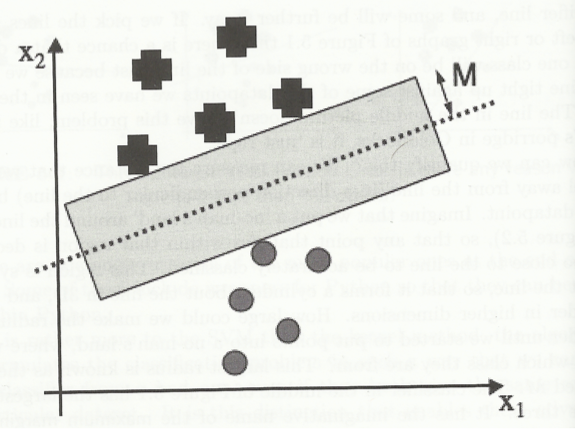
\includegraphics[height=50mm]{svm/svm_1.png}
    \caption{AND-Perzeptron und Raum (Platzhalterbild)}
    \label{fig:svm1}
\end{figure}

Einlagige Perzeptronen sind beschränkt auf die Lösung linear separierbarer Probleme. 
Ein einfaches XOR kann also nicht realisiert werden.  

Mit einem Trick, der Erhöhung der Dimension, können mehrlagige Perzeptronen auch nichtlinear separierbare Probleme lösen. 
So lässt sich bspw. das XOR-Problem in einem 3-dimensionalen Raum durch eine Hyperebene trennen.

\begin{figure}[htbp] \centering
    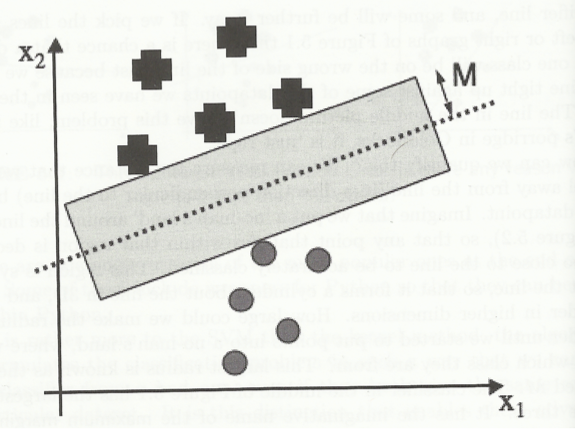
\includegraphics[height=50mm]{svm/svm_1.png}
    \caption{XOR-Perzeptron-Raum, nichtlinear separierbar (Platzhalterbild)}
    \label{fig:svm1}
\end{figure}


Die Wahl der richtigen Gewichte ist dabei nicht einfach, für komplexere Problemstellungen schier unmöglich. 
Um dennoch eine Problemlösung zu modellieren, die Eingaben richtig klassifiziert, gibt es einen Algorithmus, der die Gewichte automatisch anpasst.
Dieser Algorithmus setzt eine Trainingsmenge voraus, für dessen Eingabevektoren die zugehörigen Klassen bekannt sind. 
Durch Fehlerrückführung kann ein MLP trainiert werden und das Netz kann die gewünschten Muster nach einer kontrollierten Trainingsphase klassifizieren.

Knapp 40 Jahre Jahre später veröffentliche der sowjetisch-amerikanische Mathematiker Wladimir Wapnik \cite{Vapnik} das Prinzip der Support-Vector-Machines (SVM).

Im Gegensatz zu MLPs wird die Anpassung der Trennung nicht empirisch durch Trainingsmethoden, sondern durch die Datengrundlage mathematisch optimal ermittelt. 
Eine Erhöhung der Dimension ist nicht möglich, dennoch können SVMs auch nichtlinear separierbare Probleme lösen. 
Die Hauptidee dabei ist die Repräsentation der Daten zu verändern. 
Mit Hilfe des sogenannten Kernel-Tricks werden die Daten in einen höherdimensionalen Raum transformiert. 

Support Vector Machines erfreuen sich großer Beliebtheit, da sie in der Regel wesentlich performanter vernünftige Vorhersagen treffen können. Lediglich durch die Lokalisierung des Objekts im Koordinatensystem wird klassifiziert. Dadurch, dass eine trainierte SVM eine Trenngerade generiert, kann durch einfache Hilfsmittel aus der linearen Algebra die Position bestimmt werden. Es wird also entschieden, ob das zu klassifizierende Objekt "{}oberhalb"{} oder "{}unterhalb"{} der Trenngeraden liegt. Allerdings ist zu beachten, dass für sehr große Datenmengen die SVM eine sehr lange Trainingsphase benötigt, da der Algorithmus die Inversion der Eingabematrix benutzt. Das Bilden der inversen Matrix hat eine Laufzeit zwischen $\mathcal O(n^2)$ und $\mathcal O(n^3)$ und ist damit sehr aufwändig.


\subsection{Funktionsweise der SVM}

Mit einem Satz von Merkmalsvektoren (Merkmalsraum) und dessen Klassenzugehörigkeiten $\{ (x_1, y_1), ..., (x_m, y_m) | x_i \in \mathcal{X}, y_i \in \{-1, 1\}, m \in \mathbb{N} \}$ wird eine mathematische Gerade errechnet,
die in einem Koordinatensystem betrachtet die Daten räumlich in zwei Klassen trennt. 



Die Gerade (Hyperebene im mehrdimensionalen Raum) trennt die Merkmalsräume bestmöglich und dient als Entscheidungsfunktion für die Klassifikation. Sie ist gegeben durch den Normalenvektor $w$ und dem sogenannten Bias $b$, dem Abstand der Ebene zum Ursprung. Diese Form erweist sich also besonders praktisch, da durch Einsetzen von $x$ der direkte Abstand zur Hyperbene resultiert.
Intuitiv ist klar, dass alle Punkte auf der Hyperebene selbst keinen Abstand haben, die Formel der Hyperebene lautet demnach: 
 
\begin{equation}
\label{eq:svm_hyperplane}
    \mathcal{H}: \{ x \,|\, \langle w,x \rangle + b = 0 \}
\end{equation}
 
Allein durch das Vorzeichen der Entscheidungsfunktion ordnet die SVM die Eingabe einer Klasse zu. 

\begin{equation}
\label{eq:svm_decision0}
    \mathcal{C}_{-1}: \{ c \,|\, sign(\langle w,x \rangle + b) = -1 \}
\end{equation}

\begin{equation}
\label{eq:svm_decision1}
    \mathcal{C}_1: \{ c \,|\, sign(\langle w,x \rangle + b) = 1 \}
\end{equation}

Die nächstliegenden Vektoren zur Trenngeraden werden als Stützvektoren, der Abstand als Margin $M$ bezeichnet (Abb. XX). 
Die Stützvektoren bilden das tragende Konstrukt der Entscheidungsfunktion. 
Alle andere Merkmalsvektoren haben keinen Einfluss auf die Trennung, was die Namensgebung der Stützvektoren begründet. 
Das macht die SVM zu einem sehr transparenten und performantent Klassifikator. 


\subsubsection{Kernel-Trick}
Es ergeben sich Unregelmäßigkeiten bei der Lösung von nichtlinear separierbaren Probleme und der Klassifikation von mehr als 2 Klassen.
Im Gegensatz zu den MLPs kann man mit der Erhöhung der Dimension diesen Umstand nicht umgehen. 
Die SVMs setzen in diesem Falle auf die Transformation der Datenrepräsentation. 
Mit Hilfe von Kernfunktionen lassen sich Daten von $\mathbb{R}^n$ in einen höherdimensionalen Raum $\mathbb{R}^h$ transformieren, in dem sie linear separierbar erscheinen (Abb. XX). 

\begin{figure}[htbp] \centering
    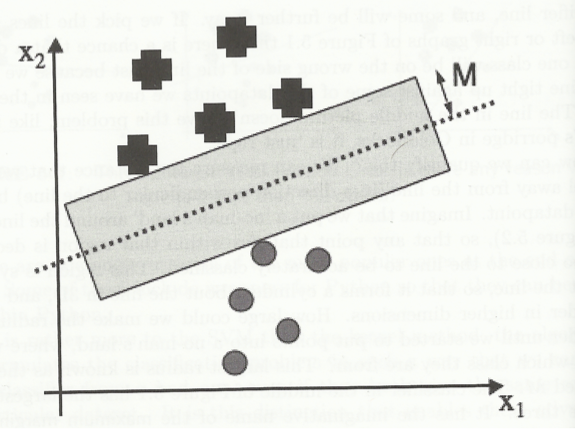
\includegraphics[height=50mm]{svm/svm_1.png}
    \caption{Die Kernel-Funktion repräsentiert die Daten in einem höherdimensionalen Raum, in dem sie linear separierbar erscheinen (Platzhalterbild)}
    \label{fig:svm1}
\end{figure}

\begin{equation}
\label{eq:svm_kernel_function}
\begin{split}
    \phi : & \mathbb{R}^n \to \mathbb{R}^h \\
    & x \mapsto \phi(x)
\end{split} 
\end{equation}

Als Bedingung des Raums $\mathbb{R}^h$ gilt, dass das Skalarprodukt erklärt ist. 
Wir haben nach der Transformation also die neue Form \ref{eq:svm_kern_tranformation}. 
In der neuen Form müssen wir nun das Skalarprodukt $\langle\phi(w),\phi(x)\rangle$ ausrechnen, was sehr schwierig (bzw. unmöglich) ist, wenn die Dimension von $\mathbb{R}^h$ zu groß wird.

\begin{equation}
\label{eq:svm_kern_tranformation}
    \mathcal{C}: \{ c_i \,|\, sign(\langle \phi(w),\phi(x) \rangle + b) = i \}
\end{equation}

Dadurch, dass die Trainingspunkte $x$ nur in Skalarprodukten auftauchen, können wir uns des Kernel-Tricks bedienen.
Kernel-Funktionen, die in $\mathbb{R}^n$ leben, zeichnen sich durch eine spezielle Eigenschaft aus, da sie sich verhalten wie ein Skalarprodukt in $\mathbb{R}^h$. 

\begin{equation}
\label{eq:svm_kern_trick}
    \mathcal{K}(w,x) = \langle\phi(w),\phi(x)\rangle
\end{equation}

Es kann also das Skalarprodukt $\langle\phi(w),\phi(x)\rangle$ in $\mathbb{R}^h$ ausgerechnet werden, ohne die Daten mittles $\phi$ zu transformieren. 
Das Beispiel XX verdeutlicht die Anwendung des Kernel-Tricks  anhand einer polynomiellen Kernfunktion:




\begin{equation}
\label{eq:svm_kernel_example}
\begin{split}
    & \text{Seien } w,x \in \mathbb{R}^2 \text{ und}\\
    \\
    \phi : & \mathbb{R}^2 \to \mathbb{R}^3\\
    & \begin{pmatrix}
    x_1 \\
    x_2
    \end{pmatrix}
    \mapsto
    \begin{pmatrix}
    x_1^2 \\
    \sqrt{x_1x_2} \\
    x_2^2
    \end{pmatrix}\\
    \\
    & \text{dann ist:}\\
    \\
    \langle \phi(w),\phi(x) \rangle = & \:\langle \begin{pmatrix}
    w_1^2 \\
    \sqrt{w_1w_2} \\
    w_2^2
    \end{pmatrix},
    \begin{pmatrix}
    x_1^2 \\
    \sqrt{x_1x_2} \\
    x_2^2
    \end{pmatrix} \rangle \\
    \\
    = & \:w_1^2x_1^2 + 2 w_1x_1w_2x_2 + w_2^2x_2^2 \\
    \\
    = & \:(w_1x_1 + w_2x_2)^2 \\
    \\
    = & \:\langle w,x \rangle^2 \overset{\text{(def)}}= \mathcal{K}(w,x)
\end{split}
\end{equation}

Nicht jede beliebige Funktion ist eine Kernelfunktion. Kernelfunktionen müssen die Bedingungen nach Satz von Mercer (MLBUCH94, S.127) erfüllen.

\begin{figure}[htbp] \centering
    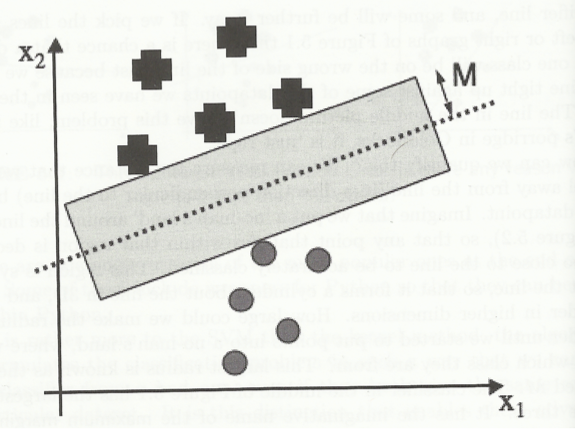
\includegraphics[height=50mm]{svm/svm_1.png}
    \caption{SVM-Räume, wx+b, M (Platzhalterbild)}
    \label{fig:svm1}
\end{figure}

\newpage

\subsection{Implementierung}

Das “scikit-learn”-Paket von den “scikit-learn developers” steht frei unter BSD License für Python zur Verfügung. 
Es beinhaltet viele komfortable Bibliotheken zum Thema Machine Learning. 
Für unsere Zwecke benutzen wir die vorgefertigten SVM-Algorithmen. 
Diese berücksichtigen freundlicherweise bereits die Features für die Klassifizierung mehrerer Klassen sowie den Kernel-Trick. Eine SVM wird folgendermaßen trainiert:

\begin{lstlisting}
import numpy as np#
from sklearn import svm#

X = np.array([[-1,1],[1,1],[1,-1],[-1,-1]])
y = [1,-1,1,-1]

#Train SVM
clf = svm.SVC(kernel='linear')
clf.fit(X, y)#

#Predict
print clf.predict([0.2,0.2])#
print clf.predict([-0.2,0.2])#
print clf.predict([-0.2,-0.2])#
print clf.predict([0.2,-0.2])#
\end{lstlisting}


\subsection{Vorverarbeitung der Eingabedaten}

Kernpunkt der Gestenerkennung ist die anliegende Grundfrequenz von 18 kHz. 
Die aktuelle Implementierung der Gestenerkennung setzt ein Audiosignal mit einer Länge von 320 ms voraus. 
Innerhalb dieser 320 ms werden 32 Merkmalsvektoren mit einer zeitlichen Dauer von 1 ms gespeichert in einem Intervall von je 10 ms. 
Diese zeitlich versetzten 32 Merkmalsvektoren mit je 64 Datenpunkten einer Geste werden vor der Eingabe in eine trainierte SVM zuerst normalisiert. 
Dazu gibt es zwei grundlegende Ansätze:

- alle 32 Merkmalsvektoren werden mit einem “globalen” Maximalwert über alle 32 Datensätze in den Bereich zwischen 0 und 1 normalisiert\newline

- alle 32 Merkmalsvektoren werden mit ihrem jeweiligen Maximalwert in den Bereich zwischen 0 und 1 normalisiert

Letztere Methode sorgt dafür, dass die Grundfrequenz der Gestenerkennung von 18 kHz in allen Merkmalsvektoren in einem Maximalwert von 1 resultiert. 
In einem nächsten Schritt bietet es sich an, diese Grundfrequenz, die ebenfalls nach der gleichen Methode normalisiert wurde, von den Merkmalsvektoren abzuziehen. 
Dadurch wird die reine Frequenzverschiebung der Geste gut sichtbar und man erhält eine sehr gute Eliminierung von Stördaten. 
Anschließend bietet es sich allerdings an, die Merkmalsvektoren erneut in den Bereich zwischen [0, 1] zu skalieren, da durch die Subtraktion der Grundfrequenz negative Werte entstehen können.


\subsection{Eingabe in die SVM}

Die zeitlich versetzten 32 Merkmalsvektoren mit je 64 Datenpunkten einer Geste können für die Eingabe in eine trainierte SVM linear aneinandergehängt werden, so dass ein einziger Eingabevektor mit 32*64 = 2048 Elementen entsteht. 
Dieses Vorgehen ist nicht kritisch, da wir die Zeitkomponente bei einer SVM nicht näher betrachten müssen. 
Sie wird indirekt durch die Position in unserem Eingabevektor berücksichtigt.

Im folgenden ist eine geplottete Aufnahmen einer Gesten zu erkennen. 
Die oberen vier Zeilen zu je acht Graphen sind die zeitlich aufeinanderfolgenden 32 Merkmalsvektoren. 
Der blaue Graph hierbei ist der normalisierte Merkmalsvektor, während die roten Graphen jeweils das Ergebnis von Merkmalsvektor - Grundfrequenz beinhalten. 
Die Grundfrequenz wurde aus insgesamt 12 verschiedenen Aufnahmen zu je 32 Merkmalsvektoren (insgesamt 384 Merkmalsvektoren) gemittelt. 
Sie ist als grüner Graph in den Bildern zu sehen.

\begin{figure}[h!]
  \centering
    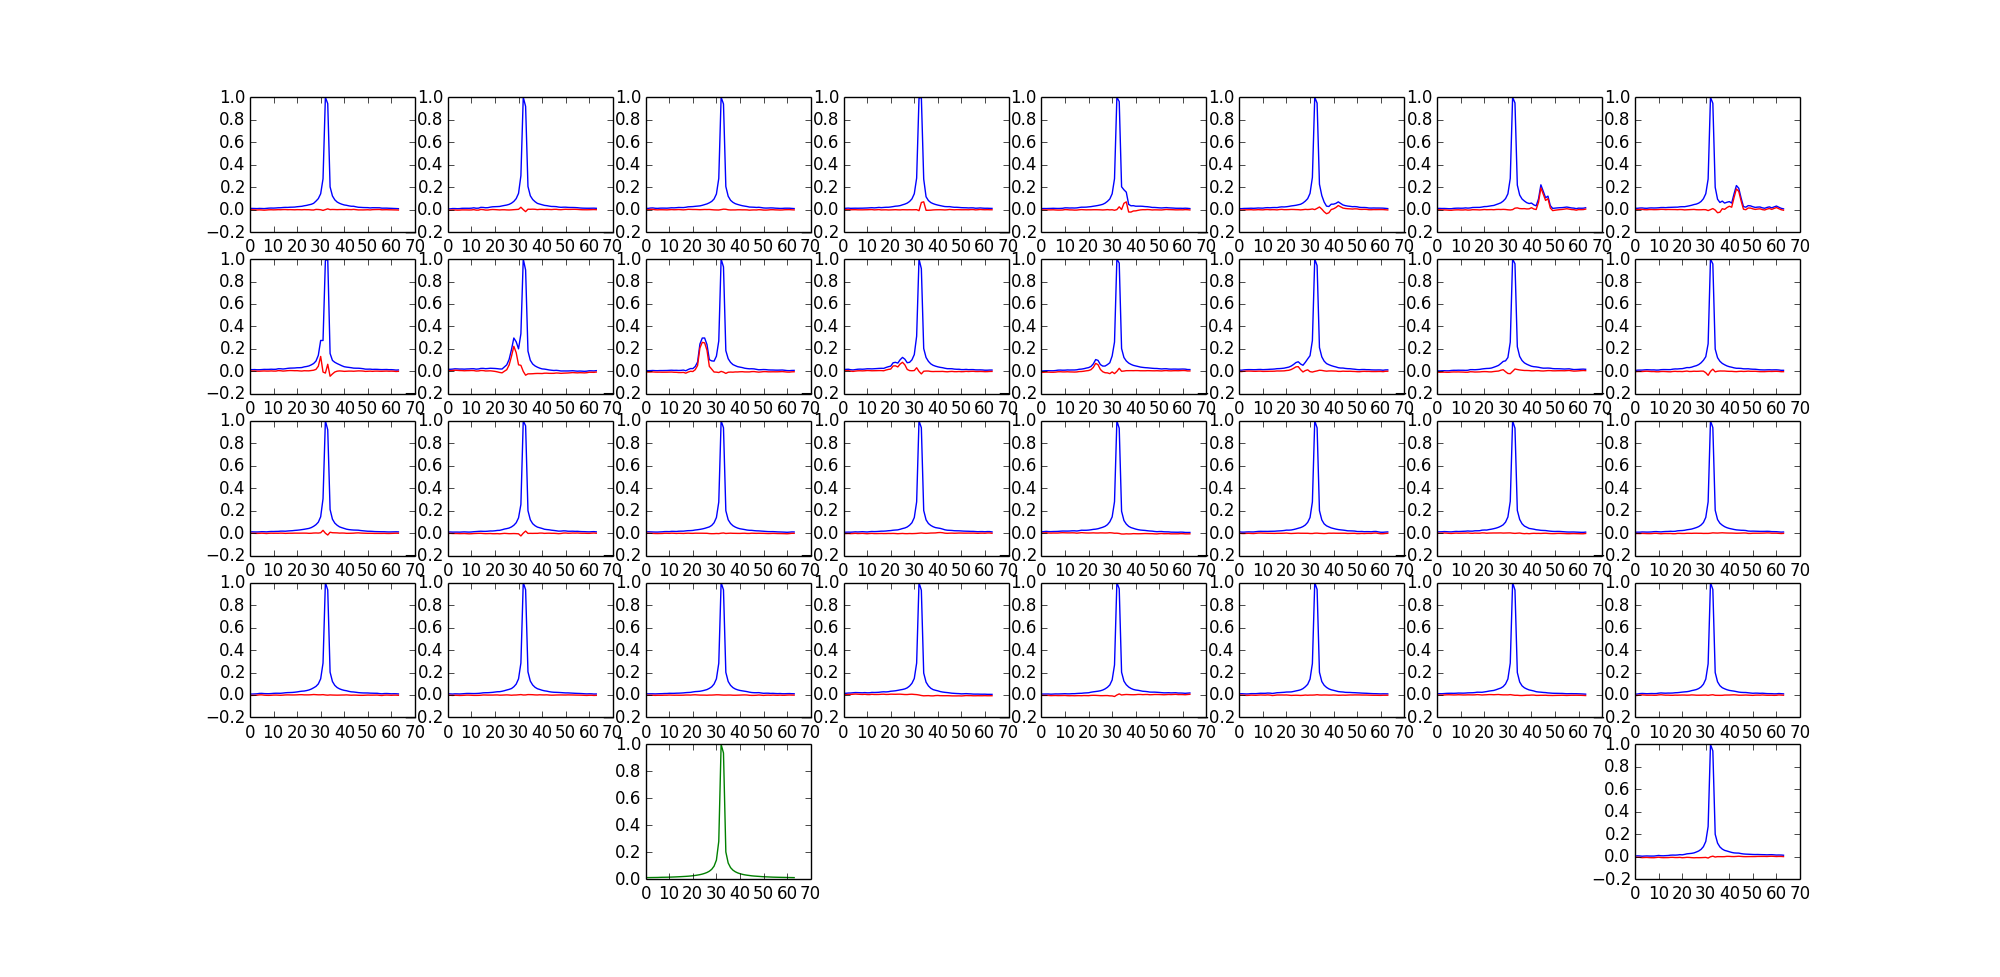
\includegraphics[width=0.8\textwidth]{svm/svm_data_1.png}
  \caption{Ausgabe der (transformierten) Merkmalsvektoren}
\end{figure}


\newpage 
\subsection{Anwendung auf das Projekt}
\begin{itemize}
\item{normierung}
\item{quantisierung}
\item{transformation}
\end{itemize}

% UND-Perzeptron

\subsubsection{Datenaufbereitung}
In Kapitel \ref{Kapitel 1 TODO} wurde die Aufnahme und die generelle Vorverarbeitung der Daten bereits erläutert, bevor diese an die entsprechenden Klassifikatoren weitergeleitet werden.
Die Klassifikatoren erhalten dabei jeweils einzelne Frames mit bereits normalisierten 64 Werten, die sich innerhab des Frequenzbereichs um die Referenzfrequenz von $18500\text{kHz}$ befinden  \{Bild einfügen\}. 
Da jeder Klassifikator aufgrund seiner Funktionsweise unterschiedlich mit den Eingabedaten arbeitet, ist eine entsprechende und auf den jeweiligen Klassifikator angepasste Datenaufbereitung notwendig.

Dieser Abschnitt befasst sich mit der spezifischen Datenaufbereitung für den Support Vector Machine Klassifikator.

[..]
Bei der Betrachtung der Trainingsdaten beziehungsweise -Gesten fällt auf, dass die durch den Dopper-Effekt verursachten Frequenzverschiebungen in einem relativ kleinen Bereich um die Referenzfrequenz herum sattfinden.
Zudem wird offensichtlich, dass nur ein Bruchteil der ursprünglich veranschlagten 32 Frames pro Geste relevante Informationen enthalten, da eine ausgeführte Geste meist zwischen 8 und 16 Frames lang ist beziehungsweise nur innerhalb dieser Frame-Anzahl Frequenzverschiebungen verursacht.
Um diesen Overhead an nicht nutzbaren Daten zu beseitigen, wird die zu betrachtende Frame-Anzahl bei der Live-Klassifikation auf 20 festgelegt.
Der verwendete Wertebereich eines Frames wird sowohl in der Trainingsphase, als auch in der Live-Klassifikation, von 64 auf 40 verkleinert \{Bild einfügen\}. 

Da nach der Vorverarbeitung der Daten (\ref{Kapitel 1 TODO} trotz Subtraktion der Referenzfrequenz teilweise noch sehr feines Rauschen in den Daten vorhanden sein kann, werden Werte unterhalb eines festgelegten Schwellenwerts (Threshold) auf 0 gesetzt.
Ein Aufsummieren aller Frames mit anschließender Normalisierung liefert ein ''Gesamtergebnis'' einer Geste, in der sich alle relevanten Merkmale befinden.

Durch die Reduzierung des Wertebereichs auf 40 Werte pro Frame und durch das Aufsummieren zu einer Einheitsgeste wird eine Problemdimensionsreduzierung beim Training einer SVM um den Faktor ~51 erzielt.
Eine weitere Reduzierung um den Faktor 2 ist möglich, sofern nur jeder zweite Wert der Einheitsgeste für das Training verwendet wird.


\subsubsection{Anpassung des Klassifikators}
- Ergebnisorientoiert

\subsubsection{Implementierung}
Aufgrund des Einsatzes von verschiedenen Klassifikatoren ist ein gemeinsames Interface für alle Klassifikatoren vorhanden, welches von jedem Klassifikator -- allerdings unterschiedlich -- implementiert ist. 
Dabei handelt es sich um die abstrakte Klasse \textit{IClassifier}.

Für die Implementierung des \ac{SVM}-Klassifikators innerhalb der Klasse SVM wird die Python-Bibliothek \cite{scikit-learn} verwendet. 
Die Bibliothek stellt neben einer Vielzahl von weiteren Modulen und Klassen unter anderem auch eine Implementierung einer SVM zur Verfügung.
Für grundlegende Matrizenberechnungen wird die Python-Bibliothekt \cite{NumPy} verwendet. \cite{NumPy} zeichnet sich vor allem durch effiziente Berechnungsoperationen und eine Vielzahl an nützlicher Funktionen aus.
Zusätzlich findet das in der Python-Installation enthaltene \cite{subprocess}-Modul Einsatz, um mittels erkannter Gesten verschiedene Programme starten und beenden zu können.

Die Methode \textit{classify} führt die entsprechenden Vorverarbeitungsschritte pro übergebenem Frame aus und speichert diesen in einer globalen Liste \textit{self.datalist}. 
Mittels einer Abfrage, ob der Frame überhaupt relevante Informationen besitzt, wird der Gestenanfang erkannt und der entsprechende Index der Liste \textit{self.datalist} gespeichert.
Sobald 20 weitere Frames in dieser Liste abgespeichert worden sind, startet zunächst ein weiterer Vorverarbeitungsschritt, in dem alle Frames zu einer Einheitsgeste aufsummiert werden.
Die normalisierte Einheitsgeste ist das finale Ergebnis der Vorverarbeitung der Live-Klassifikation und dient dem SVM-Klassifikator als Eingabedatum.
Als Rückgabewert liefert der Klassifikator die entsprechende Gestennummer, die er dem Eingabedatum zugeordnet hat.
Mittels dieser Nummer wird eine Methode aufgerufen, in der jeder Nummer eine entsprechende Funktion zugeordnet ist.

\begin{lstlisting}[language=Python,caption={Classify},label={lst:svm_classify}]{lst:svm_classify}
def classify(self, data):
	# init num samples per frame and borders
	sliced_num_samples_per_frame = SVM.NUM_SAMPLES_PER_FRAME - SVM.SLICE_RIGHT - SVM.SLICE_RIGHT
	left_border = SVM.SLICE_LEFT
	right_border = SVM.NUM_SAMPLES_PER_FRAME - SVM.SLICE_RIGHT

	normalized_data_with_noise = data / np.amax(data)
	normalized_data = normalized_data_with_noise[left_border:right_border] - self.noise_frame[
																			 left_border:right_border]

	frame = normalized_data
	irrelevant_samples = np.where(frame <= 0.025)
	frame[irrelevant_samples] = 0.0

	rr = 20  # whats that?!?
	self.datalist.append(frame)
	self.datanum += 1

	if np.amax(frame) > 0.0 and self.found == False:
		self.index = self.datanum
		self.found = True

	if self.index + rr == self.datanum and self.found == True:
		self.index = 0
		self.found = False

		current_frameset = np.asarray(self.datalist[-rr:])
	
		gesture_frame = current_frameset.sum(axis=0)

		try:
			normalised_gesture_frame = gesture_frame / np.amax(gesture_frame)
			if not np.isnan(np.sum(normalised_gesture_frame)):
				target_prediction = self.classifier.predict(normalised_gesture_frame[::2])[0]  # only each second?!?
				self.executeCommand(target_prediction)
		except:
			print "error =("

	if self.datanum > sliced_num_samples_per_frame:
		del self.datalist[0]
\end{lstlisting}


\begin{lstlisting}[language=Python,caption={Start Programms},label={lst:svm_startprogramms}]{lst:svm_startprogramms}
def executeCommand(self, number):
	print number,

	if number == 0 and self.executed["notepad"] == False:
		print "starting notepad"
		proc = sp.Popen("notepad")
		self.executed["notepad"] = proc.pid

	elif number == 1 and self.executed["notepad"] != False:
		sp.Popen("TASKKILL /F /PID {pid} /T".format(pid=self.executed["notepad"]))
		print "terminating notepad"
		self.executed["notepad"] = False

	elif number == 2 and self.executed["taskmgr"] == False:
		print "starting taskmanager"
		proc = sp.Popen("taskmgr")
		self.executed["taskmgr"] = proc.pid

	elif number == 3 and self.executed["taskmgr"] != False:
		sp.Popen("TASKKILL /F /PID {pid} /T".format(pid=self.executed["taskmgr"]))
		print "terminating taskmanager"
		self.executed["taskmgr"] = False

	elif number == 4 and self.executed["calc"] == False:
		print "starting calculator"
		proc = sp.Popen("calc")
		self.executed["calc"] = proc.pid

	elif number == 5 and self.executed["calc"] != False:
		sp.Popen("TASKKILL /F /PID {pid} /T".format(pid=self.executed["calc"]))
		print "terminating calculator"
		self.executed["calc"] = False

	elif number == 6:
		print "noise, do nothing ..."

	print ""
\end{lstlisting}


\subsubsection{Training}
- Trainingsmethode